
\chapter{Physical Layer Components}

In Chapter~\ref{ch:repeaters}, we saw the basics of a quantum repeater and how it can distribute entanglement over long distances. In this chapter, we will go a little bit deeper and see how individual physical components of a quantum repeater work.

\section{Introduction}

\begin{figure}[t]
    \centering
    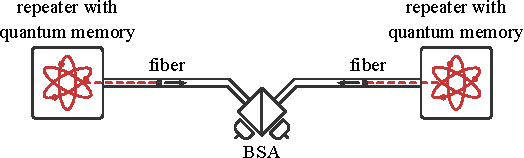
\includegraphics[width=0.7\textwidth]{lesson13/13-1_repeater.pdf}
    \caption[MIM link hardware]{An MIM link. The nodes at each end are repeaters with memories, shown by the atom symbols.  The node in the middle is the Bell-state analyzer (BSA).  The red circles represent photons in flight, entangled with the memories.}
    \label{fig:13-MIM-link}
\end{figure}


Fig.~\ref{fig:13-MIM-link} shows the basic architecture for a quantum repeater link.
We have our two network nodes, represented by the boxes, each of which contains one or more qubits represented by the atom symbols.
The qubits emit photons toward the middle node, which implements a Bell-state measurement.
That way, we can establish entanglement over long distances. What are the individual physical components of a quantum repeater system, and more importantly how can we implement them? First, we need optical fibers to carry our photons. That's kind of obvious, and already we have covered optical fibers at some length in Chapters~\ref{sec:7_waveguides}\index{optical fiber} and \ref{sec:11_long-distance}. Next, we need the Bell-state analyzer in the middle. The analyzer implements our Bell-state measurement, which is crucial for implementing entanglement swapping.

While the photons are in flight and traveling toward our Bell-state analyzer (BSA)\index{Bell-state analyzer (BSA)}, the qubits stored in the nodes are stationary. They are not moving anywhere, so we must have some physical means of storing these qubits, which we do with the help of \emph{quantum memory}\index{quantum memory}. The difference between classical memories and quantum memories is quite substantial. Classical memories store zeros and ones (classical bits), whereas quantum memories have to be able to store not only one or zero, but also any superposition, and in fact any entangled state. 
%That way, they can share entanglement over the entire quantum network. 
After talking about the two basic components of BSAs and memories, we will consider how all of these components work together to implement a quantum repeater. Most importantly, we will also consider the various factors that affect the success rate of our quantum repeater and entanglement swapping scheme. We will spend the first half of this chapter talking about Bell-state analyzers. We will revisit measurements and how they can actually be implemented, what it means to measure in different bases, and how can we implement different basis measurements with Pauli $Z$ measurements and some unitaries. Then, we will move on to the quantum circuit for a Bell-state measurement, and from that we will talk about real-world implementation of Bell-state measurements with linear optics.  In the latter half of this chapter we will talk about memories. We will begin with consideration of what a good quantum memory should be like, then we'll move on to the candidate systems.  We say "candidate" because at the moment, there is no leading physical system that is considered to be the best quantum memory. All of the existing candidate systems have some advantages and some drawbacks.



\section{Bell State Measurements I}

% \rdv{this par needs work, but I haven't decided what to do with it. Do we really need to repeat the Bell states here?}
% Let's remind ourselves of some of the characteristics of Bell states.
% The Bell states are orthonormal. If we take the inner product of a Bell state with itself, then we get one, which means that it is normalized. But if we take the inner product of one of the Bell states with a different Bell state, then we get zero. For example, the inner product between \ket{\Phi^-} and \ket{\Phi^+} is zero, and so on,
% \begin{equation}
% \begin{aligned}
% &\left\langle\Phi^{+} \mid \Phi^{+}\right\rangle=1 \\
% &\left\langle\Phi^{-} \mid \Phi^{+}\right\rangle=0.
% \end{aligned}
% \end{equation}

% Since the Bell states are orthonormal and completely cover the possible space of two qubits, we can take any pure state of two qubits, and write it out in terms of Bell states, which we call writing it in the Bell basis\index{Bell basis}. For example, let's consider a general pure two-qubit state in the computational basis with probability amplitudes given by $\alpha$, $\beta$, $\gamma$, and $\delta$,
% \begin{equation}
% |\psi\rangle=\alpha|00\rangle+\beta|01\rangle+\gamma|10\rangle+\delta|11\rangle.
% \end{equation}

% Back in Ch.~\ref{sec:8-2_teleportation_protocol}, in the context of teleportation, we saw how to rewrite the computational basis states \ket{00}, \ket{01}, \ket{10} and \ket{11} in the Bell basis. Now we have a general two-qubit state, which is of course a superposition of the four Bell states, where naturally the probability amplitudes have changed. For example, the probability amplitude for state \ket{\Phi^+} is $(\alpha+\beta)/\sqrt{2}$, and so on for the other Bell states,
% \begin{equation}
% |\psi\rangle=\frac{\alpha+\beta}{\sqrt{2}}\left|\Phi^{+}\right\rangle+\frac{\alpha-\beta}{\sqrt{2}}\left|\Phi^{-}\right\rangle+\frac{\gamma+\delta}{\sqrt{2}}\left|\Psi^{+}\right\rangle+\frac{\gamma-\delta}{\sqrt{2}}\left|\Psi^{-}\right\rangle
% \end{equation}

% We have been treating measurement as a question that we ask about the state of our physical system, namely, which of the four Bell states is our state in? Is it the state \ket{\Phi^+}? Is it the state \ket{\Phi^-}, \ket{\Psi^+}, or \ket{\Psi^-}? This is what the measurement reveals about our system, and usually we say that we get the answer with some probability. For example, depending on the initial state \ket{\psi}, we might get the answer that the state is \ket{\Phi^+}. In this case, that answer would occur with a probability which is the modulus squared of the original complex probability amplitude,
% \begin{equation}
% \operatorname{Prob}\{\ket{\Phi^+}\}=\left|\frac{\alpha+\beta}{\sqrt{2}}\right|^2.
% \end{equation}
% This is a very abstract notion of what a measurement actually is, and it's not \rdv{?} very useful when it comes to doing calculations. Shortly, we will see how to actually implement such a measurement in terms of a quantum circuit, which will tell us more about what these measurements are actually doing and how we can implement them in a laboratory.

In this Section, we focus on the Bell state analyzer from Fig.~\ref{fig:13-MIM-link}, particularly how one can perform measurements in the Bell basis.
We have seen how to describe this measurement mathematically in Chapter~\ref{sec:4_entanglement}.
However, this tells us little about a real-world implementation.
The first step is to break down the Bell state measurement into more elementary operations in order to understand how we can implement it using a real physical system.

Let's step back a little and consider something simpler first, like measuring a single qubit in the Pauli $Z$ basis, depicted in the left panel of Fig.~\ref{fig:13-2_measurementPauli}.
The meter icon represents a measurement in the Pauli Z basis which outputs a single classical bit $c$.
The value of this classical bit can be either +1 or -1, which is normally written as $c\in\{+1,-1\}$.
For an arbitrary initial state $|\psi\rangle = \alpha |0\rangle + \beta |1\rangle$, the probability that the measurement outcome is $c=+1$ is given by $\text{Pr}(+1)=|\langle0|\psi\rangle|^2=|\alpha|^2$.
On the other hand, probability that the measurement outcome is $c=-1$ is given by $\text{Pr}(-1)=|\langle1|\psi\rangle|^2=|\beta|^2$.

\begin{figure}[t]
    \centering
    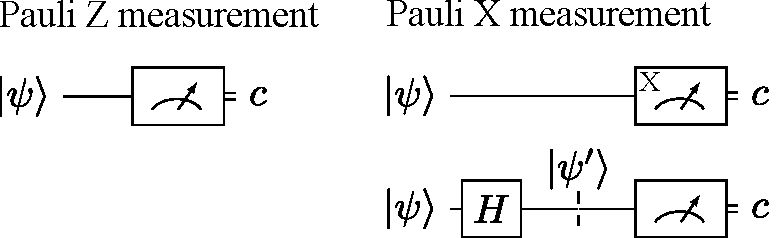
\includegraphics[width=0.6\textwidth]{lesson13/13-2_measurementPauli.pdf}
    \caption[Changing the basis of measurements.]{Changing the basis of measurement can be achieved by applying a suitable unitary and then measuring in the Pauli $Z$ basis.}
    \label{fig:13-2_measurementPauli}
\end{figure}

We can also measure the qubit in the Pauli $X$ basis as shown in the top part of the right panel in Fig.~\ref{fig:13-2_measurementPauli}.
The measurement icon includes an X to remind us that we are measuring in the Pauli $X$ basis.
Probability that we obtain $c=+1$ is $\text{Pr}(+1)=|\langle+|\psi\rangle|^2=|\alpha+\beta|^2/2$, and the probability of the outcome $c=-1$ is $\text{Pr}(-1)=|\langle-|\psi\rangle|^2=|\alpha-\beta|^2/2$.

But what if we cannot perform of the Pauli $X$ measurement directly?
Sometimes, in an experiment, it is straightforward to implement a Pauli $Z$ measurement, but much less clear how to perform a measurement in a different basis.
We can still measure in the desired basis by rotating the state with an appropriate unitary and then performing a measurement in the Pauli $Z$ basis.
In hte case of a Pauli $X$ measurement, the appropriate unitary is a Hadamard gate $H$ as shown in the lower part of the right panel in Fig.~\ref{fig:13-2_measurementPauli}.
The state immediately before the measurement in the Pauli $Z$ basis is
\begin{align}
    |\psi'\rangle & = H|\psi\rangle = \alpha |+\rangle + \beta |-\rangle \nonumber\\
    & = \frac{\alpha + \beta}{\sqrt{2}} |0\rangle + \frac{\alpha - \beta}{\sqrt{2}} |1\rangle.
\end{align}
We can immediately see that the probabilities of obtaining measurement outcomes +1 or -1 are the same as measuring in the Pauli $X$ basis directly.

How do we know that the unitary that is needed is the Hadamard $H$?
The trick lies in realizing that the probability of obtaining the $c=+1$ outcome via a direct Pauli $X$ measurement must by the same as first rotating the state with some unitary operation $U$ and then measuring in Pauli $Z$ basis.
Written more formally, we require that
\begin{equation}
    |\langle+|\psi\rangle|^2 = |\langle0|U|\psi\rangle|^2.
    \label{eq:13-2_prob_condition}
\end{equation}
Eq.~(\ref{eq:13-2_prob_condition}) is satisfied when $\langle+|=\langle0|U$, or $|+\rangle=U^{\dagger}|0\rangle$ if you prefer to think in terms of kets rather then bras.
The same unitary $U$ must also satisfy
\begin{equation}
    |\langle-|\psi\rangle|^2 = |\langle1|U|\psi\rangle|^2,
\end{equation}
that is the probabilities of obtaining the outcome $c=-1$ via direct measurement in Pauli $X$ basis and via rotating the state before measuring in the Pauli $Z$ basis must be the same.
The unitary operation $U$ that achieves this transformation is the Hadamard $H$ as we have seen in Sec.~\ref{sec:2-2_unitary_operations}.

\begin{figure}
    \centering
    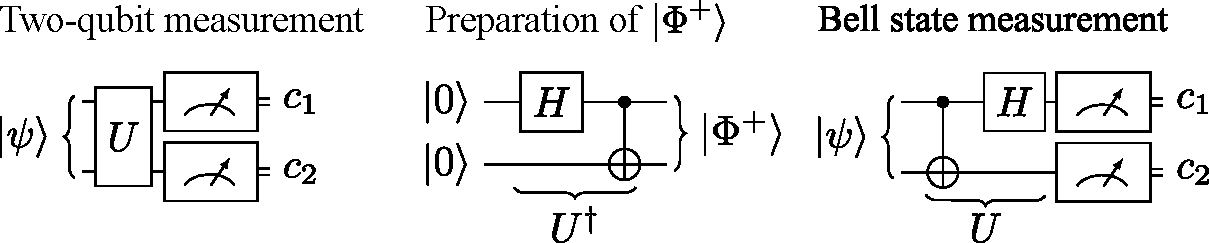
\includegraphics[width=0.9\textwidth]{lesson13/13-2_measurementBell.pdf}
    \caption[Bell state measurement via Pauli Z measurements]{Performing the Bell state measurement can be achieved by the right unitary $U$ followed by two measurements in the Pauli $Z$ basis.}
    \label{fig:13-2_measurementBell}
\end{figure}

Transforming the measurement basis by applying a suitable unitary operation on the state does not stop with single qubits but works for multi-qubit measurements as well.
Let's finally turn our attention to the Bell state measurement.
What is the two-qubit unitary that we must apply such that subsequent measurements of both qubits in the Pauli $Z$ basis have the same effect as a Bell state measurement?
We can apply the same technique that we used in the case of single-qubit Pauli $X$ measurement and look for a unitary $U$ which satisfies
\begin{equation}
    |\langle\Phi^+|\psi\rangle|^2 = |\langle00|U|\psi\rangle|^2,
\end{equation}
where $|\psi\rangle$ is now an arbitrary two-qubit state, as depicted in the left panel of Fig.~\ref{fig:13-2_measurementBell}.
The outcomes of the measurements on the first and second qubit are denoted by $c_1$ and $c_2$, respectively.
We see that our desired unitary $U$ must satisfy $\langle\Phi^+| = \langle00|U$, which can be expressed in the ket notation by taking the adjoint of both sides,
\begin{equation}
    |\Phi^+\rangle = U^{\dagger} |00\rangle.
\end{equation}
This means we need to find the unitary $U^{\dagger}$ which transforms the input $|00\rangle$ into the Bell pair $|\Phi^+\rangle = (|00\rangle + |11\rangle) / \sqrt{2}$.
This unitary operation is pictured in hte middle panel of Fig.~\ref{fig:13-2_measurementBell},
\begin{equation}
    U^{\dagger} = CNOT_{12} \cdot (H \otimes I)
    \label{eq:13-2_Uadjoint}
\end{equation}
Starting from the initial state where both qubits are initialized in the $|0\rangle$, we need to apply the Hadamard operation $H$ to the first qubit, followed by a controlled-NOT gate with the first qubit being the control and the second qubit the target.
All that remains to be done is to take the adjoint of Eq.~(\ref{eq:13-2_Uadjoint}),
\begin{equation}
    U = (H \otimes I) \cdot CNOT_{12}.
\end{equation}
This is the unitary operation that we need to apply to state in order to be able to perform a Bell state measurement using measurements in the Pauli $Z$ basis as shown in the right panel of Fig.~\ref{fig:13-2_measurementBell}.
This trick is very useful in both quantum computation and quantum communication.



\section{Bell State Measurements II}
\label{sec:13-3_Bell_state_measurement_2}

In this section, we will talk about how to implement a Bell-state measurement with linear optics. The implementation scheme depends on the encoding. Let's encode the state of a qubit using the photon polarization. There are two reasons for this choice: first, it's intuitive and simple so it makes a good pedagogical example, and second, it's one of the most commonly used encodings in real experiments.

In this encoding, qubit in a state \ket{0} is represented as a single photon that is polarized in the horizontal direction, which we write as \ket{H}.
Our other computational basis state \ket{1} is represented as a single photon polarized in the vertical direction, and we write \ket{V}.

\begin{figure}[t]
    \centering
    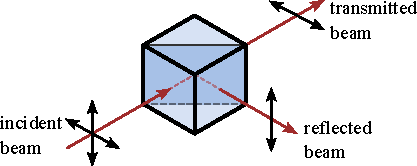
\includegraphics[width=0.6\textwidth]{lesson13/13-3_PBS.pdf}
    \caption[A polarizing beam splitter (PBS)]{The action of a polarizing beam splitter (PBS).  The vertical rays represent vertically polarized light \ket{V}, while the diagonal rays represent horizontally polarized light \ket{H}.  The direction of propagation, red arrows, is normal to the \ket{H}-\ket{V} plane.}
    \label{fig:13-PBS}
\end{figure}

The first question that we should ask is, "how do we implement a Pauli $Z$ measurement with this encoding"? We have to measure and distinguish the two different polarizations, horizontal and vertical. That can be done with a little piece of crystal called a \textit{\textbf{polarizing beam splitter}} (PBS)\index{polarizing beam splitter (PBS)}, as shown in Fig.~\ref{fig:13-PBS}. If we have a beam of light coming in with some polarization, a PBS splits the beam of light into two beams. One beam is transmitted through the polarizing beam splitter but comes out only with a horizontal polarization, while the other beam gets reflected by the PBS and is polarized in the vertical direction. The relative strength of the two beams naturally depends on the polarization of the input light; the PBS is not creating or changing polarization, but rather sorting the input light into the two categories.
Thinking in terms of computational states, we now have two beams, one for our \ket{0} and one for our \ket{1}.

\begin{figure}[t]
    \centering
    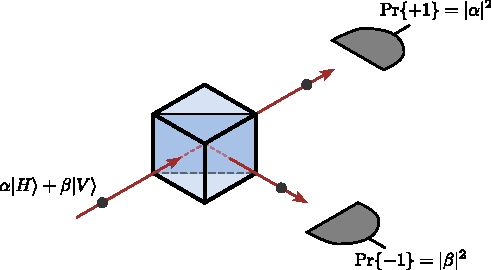
\includegraphics[width=0.7\textwidth]{lesson13/13-3_PBS_measure.pdf}
    \caption[A polarizing beam splitter (PBS) measuring a qubit]{A PBS measuring an arbitrary photonic qubit in the \{$|H\rangle$, $|V\rangle$\} basis.}
    \label{fig:13-PBS-measure}
\end{figure}

Assume that we have a single photon polarized in the vertical direction, and we place two detectors after the polarizing beam splitter to detect which output path was taken by the single photon. If the photon is horizontally polarized, it gets transmitted through the polarizing beam splitter.
Therefore, it gets detected by the detector placed in the transmitted path with probability one.
This represents our measurement outcome of $+1$. Since the photon is horizontally polarized, no vertically polarized photon is present to come out of the reflected path and trigger that detector, so the probability of the outcome $-1$ is 0.
On the other hand, if the initial photon is vertically polarized, it always gets reflected and travels down into the bottom detector, where it always gets detected.
In that case, the probability of the outcome $-1$ is 1, and the probability of the outcome $+1$ is always 0.

What happens if we put in a superposition of the two linear polarizations, as in Fig.~\ref{fig:13-PBS-measure}?
Our input state is given by $\alpha\ket{H} + \beta \ket{V}$.
The photon has a chance to get transmitted, with probability given by $|\alpha|^2$, and it also has a chance to get reflected and travel down into the other detector corresponding to the measurement outcome $-1$ (bottom), with probability of $|\beta|^2$.
This arrangement implements a $Z$ measurement.

We have seen in the previous step that for a Bell-state measurement, we need two measurements in the $Z$ basis and a suitable unitary.
Let's see what happens when we take two sub-units like the one in Fig.~\ref{fig:13-PBS-measure} and join them with a regular (not polarizing) 50/50 beam splitter, as in Fig.~\ref{fig:13-BSA-clicks}. Assume we have two photons, one coming from the top and one coming from the left, and they arrive at the beam splitter at the same time.
A complete analysis would require a little bit more quantum optics than we have studied so far, so instead of the full derivation, here we will give the result. Depending on which of the four detectors click, we may learn which Bell-state has been measured. Let's see what the different patterns are.

\begin{figure}[t]
    \centering
    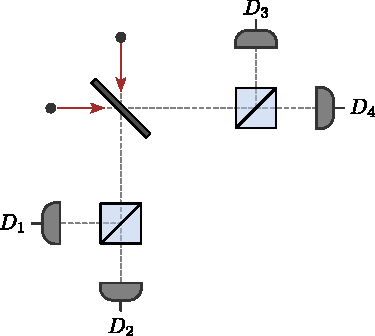
\includegraphics[width=0.6\textwidth]{lesson13/13-3_BSA_clicks.pdf}
    \caption[A four-detector Bell-state analyzer (BSA)]{A BSA measuring a pair of photonic qubits, one arriving at the initial beam splitter from above and one from the left.  Different click patterns on the four detectors may confirm projection of the pair into a Bell state, or be ambiguous.}
    \label{fig:13-BSA-clicks}
\end{figure}

If we get a joint detection in detectors $D_1$ and $D_4$, meaning that both detectors click, then we have implemented a successful Bell measurement, and the outcome corresponds to the projection onto the state \ket{\Psi^-}. If we get a joint detection in $D_2$ and $D_3$, then we can also say that we have implemented a successful Bell measurement, and the result corresponds to the state \ket{\Psi^-}. A different pattern is a joint detection at the two detectors in the lower branch of our Bell-state analyzer (both $D_1$ and $D_2$ click), from which we can conclude that we have a state \ket{\Psi^+}, corresponding to another successful Bell measurement. Equally, if both detectors in the right branch of our Bell-state analyzer ($D_3$ and $D_4$) click, then we can also conclude that we have a Bell-state \ket{\Psi^+}.

It is also possible that both photons travel into a single detector. (Detection in any of the four detectors is equally probable.) However, because more than one Bell state can result in this happening, the answer we get is ambiguous: we cannot say that whether we have \ket{\Phi^+} or \ket{\Phi^-}.
%So whenever we get only one of these detectors triggered, then we know that we have one of the state \ket{\Psi^+} or \ket{\Psi^-}, but we cannot tell which one. 
This is a bit of a problem because we cannot fully implement a Bell-state measurement. We cannot distinguish all four Bell states, only two of them, \ket{\Psi^+} and \ket{\Psi^-}.

\begin{table}
\centering
\begin{tabular}{p{0.55in}|c|p{1.5in}|c}
pattern  & result & reason & action \\\hline
$D_1$ and $D_4$ & \ket{\Psi^-} & & keep and use \\
$D_2$ and $D_3$ & \ket{\Psi^-} & & keep and use \\
$D_1$ and $D_2$ & \ket{\Psi^+} & & keep and use \\
$D_3$ and $D_4$ & \ket{\Psi^+} & & keep and use \\
any single click & \ket{\Phi^\pm} (amb.)  & two photons together, or only one arrived & discard \\
no click & (N/A) & photons lost, detection failure & discard \\
any other pattern & (N/A) & detection error & discard
\end{tabular}
\caption{4-detector BSA click patterns and their outcomes, based on Fig.~\ref{fig:13-BSA-clicks}. amb., ambiguous}
\label{tab:bsa-clicks}
\end{table}

A complete, unambiguous Bell-state measurement cannot always be successfully implemented with linear optics. In fact, even with 100\% probability of receiving both photons, the maximum probability of a successful Bell measurement is limited to only 50\%.  Of course, as we saw when discussing the loss of photons in fiber, the loss of one or both photons is highly probable, increasing the ambiguity of interpreting the result of one click.  These cases (along with the case where something goes wrong in the hardware) are summarized in Tab.~\ref{tab:bsa-clicks}. 
%We have seen in a previous chapter that quantum repeaters have to contend with a lot of noise. To deal with that noise, we have to purify our states. We have also seen in previous chapters that we have to deal with lossy fibers, which was the original motivation to develop quantum repeaters. But even if we take away all of these sources of error, there is still a fundamental error in the fact that Bell-state measurement cannot be always successfully executed with linear optics. 
Moreover, we have to take into account that the two photons coming into our Bell-state analyzer have to be synchronized. If they come in so close together that two detectors click \emph{almost} simultaneously, but not close enough that the photons are truly indistinguishable, we may misinterpret the result. The Bell-state measurement has failed and we did not establish entanglement between the network nodes, but may not realize it; when we accumulate statistics about the link, this results in lowered fidelity.


\section{Stationary and flying qubits}

First, let's begin talking about what factors matter -- what does a good memory look like, and what requirements should it satisfy?  We will start with the \emph{DiVincenzo criteria}\index{DiVincenzo criteria}. These criteria were introduced in the context of quantum computation, but they also apply in the context of quantum networking, with slightly different emphasis on which ones are important.  The extended list of these criteria, with five for quantum computing and two more for quantum communication, is:

\begin{enumerate}
    \item Well-defined qubit
    \item Can be initialized
    \item Long lifetime
    \item Universal gate set
    \item Efficient measurement
%For communications, we also want:
    \item Convert or entangle stationary \& flying qubits
    \item Able to carry flying qubits long distances
\end{enumerate}

First, if we want to build a good quantum computer, we need a well-defined qubit. Now, qubits don't come for free in nature. Usually, we have very complicated systems with many different energy levels. In order to have a well-defined qubit, we must be able to take a system for which we can address two of those energy levels, distinguish them and control them as a pair, without slipping into the other energy levels.  (Sometimes a third level is used as a temporary state to achieve certain effects such as emitting a photon, but the computation is done by restricting actions to the two levels we want to use.)

Second, we need to be able to initialize this qubit. Initialization is important because then we know exactly the state from which our quantum computation begins. If we have a good procedure for initializing our qubit, we are much more likely to carry out good quantum computation.  (This initialization also sometimes involves the temporary use of a third state.)

Third, we want long lifetimes, meaning that when we put our qubits in a superposition of states, they don't decohere very quickly. Long lifetimes allow us to carry out longer and longer quantum computations, which of course we need if we want to solve harder and harder problems.  This criterion is especially important in quantum networking, as we will see below.

Fourth, we must be able to implement a universal set of gates. Our qubit and our physical system typically have a couple of ways that the bit can be manipulated, with a parameter for how long we turn on the effect.  This set needs to be designed such that they can collectively produce an arbitrary unitary evolution. If we can rotate any point on the Bloch sphere to any other point and we can entangle two qubits, that is enough.

Fifth, of course, we need efficient measurements. Just carrying out transformations of the state in a quantum manner is not enough, we somehow we must extract the information at the end of the quantum computation.

In the context of quantum communication, we have two more requirements to consider. The first of these is conversion or entanglement between stationary and flying qubits, which we already saw earlier in this chapter. Stationary qubits are those qubits that are sitting in our quantum network nodes, loaded into the quantum memories.
%They don't really move, which is why we call them stationary. 
Flying qubits are those qubits that are used for entanglement swapping in the BSAs to create link level entanglement between between the quantum memories. We must be able to entangle photons (the flying qubits) with the stationary qubits inside the memories, but also we must be able to use entanglement swapping to create end-to-end entanglement.

Lastly, we also must be able to transport flying qubits over long distances.

Here, we will look at memory lifetime and the two communications requirements.

Why is memory lifetime important? In computers, if our memory lifetime is long and our gate speeds are fast, we are able to implement longer, more complex computations.  Thus, the ratio of gate speed to memory lifetime is an important factor. In the context of quantum communication, we often store qubits for long periods of time without acting on them, as we await messages from partners in the network.  Therefore, what's really important is not the gate speed itself, but the ratio of memory lifetime to communication time, 
provided that the gate time is short compared to the round trip time (RTT). 

Let's consider how we establish link level entanglement. We start with quantum memories, and they emit photons. These photons are entangled with the memories, and they travel to a Bell state analyzer that is halfway between the quantum nodes. The BSA performs a Bell-state measurement, but then it communicate classically back to the nodes about the outcome of the Bell-state measurements. The photon going one way and the classical message returning is our node-to-BSA round trip time~\footnote{RTT for a link can be node to BSA and back again in some contexts, or all the way memory node to memory node and back again in others. It should be clear from the context which we mean.}. If our memory lifetime is shorter than the RTT, then we cannot really do much. Even if we successfully perform the Bell-state measurements on those photon pairs, by the time the return messages are received, our memories will have decohered and are not useful anymore.

To give an idea of the latencies that we're talking about, see Tab.~\ref{tab:rtt}. The speed of light in a fiber is approximately $0.2$ meters per nanosecond,
%two hundred millimeters per nanosecond, 
so if our nodes are one kilometer apart, one round trip from one node to the other and back takes ten microseconds. For a hundred kilometers, it increases to one millisecond, and for ten thousand kilometers it goes all the way up to a hundred milliseconds (0.1 seconds) per round trip time.  The values \emph{five nanoseconds per meter one way} and \emph{10 microseconds per km round trip} are easy metrics to remember.

\begin{table}
\centering
\begin{tabular}{l|r}
distance (km)  & RTT in fiber \\\hline
1     & $10\mu$sec \\
10    & $100\mu$sec \\
100   & $1$msec \\
1,000 & $10$msec \\
10,000 & $100$msec
\end{tabular}
\caption{Round trip times in optical fiber.}
\label{tab:rtt}
\end{table}

What processes degrade our memories? The two main processes are \emph{energy relaxation}\index{energy relaxation} and \emph{dephasing}\index{dephasing}, and they are characterized by two different time scales, referred to as the $T_1$ time\index{$T_1$ time} scale and the $T_2$ time\index{$T_2$ time} scale.  $T_1$ characterizes the energy relaxation time, whereas $T_2$ gives us the characteristic dephasing time. First, let's consider the energy relaxation time given by $T_1$.

\begin{equation}
\begin{aligned}
&T_1:|1\rangle \rightarrow|0\rangle \\
&\operatorname{Prob}(\ket{1})=e^{-t / T_1}
\end{aligned}
\end{equation}

This basically tells us how quickly our qubit decays from the excited state to the ground state, or from state \ket{1} into state \ket{0}. If we initialize our state in \ket{1}, the probability that after some time $t$ we still find it in the state \ket{1} is given by the expression $e^{-t/T_1}$. The probability that after $T_1$ seconds we still find our state in \ket{1} is given by $\frac{1}{e}$. This process of going from \ket{1} to \ket{0} captures the fact that usually \ket{1} is encoded into a state of our quantum memory that has a higher energy, while \ket{0} in a lower-energy state such as the ground state. (Of course that choice is by convention, not an immutable fact of physics.)  That's why we call $T_1$ the energy relaxation time.

The dephasing time gives us the time scale for the loss of phase coherence in our qubit. If we are only use qubits to implement classical communication,  $T_1$ is important but  $T_2$ not so much, because there is no quantum coherence and we are not using superpositions. But in quantum networking and quantum communication, superpositions are crucial, and those superpositions can be destroyed by this dephasing process.

If we start in an equal superposition of \ket{0} and \ket{1} (the \ket{+} state), $T_1$ is the characteristic time scale that tells us when we will end in a completely mixed state,
\begin{equation}
\begin{aligned}
\rho_{\textrm{completely mixed}} =\frac{\ketbra{0}{0}+\ketbra{1}{1}}{2}.
\end{aligned}
\end{equation}
In Sec.~\ref{sec:3-3_density_matrices}, we saw the crucial difference between complete mixtures and equal superpositions. Here, if we prepare the state in the pure state, after some time $t$ we will have the mixed state
% $T_2:|+\rangle \rightarrow$ completely mixed state
\begin{equation}
\begin{aligned}
\rho=P|+\rangle\langle+|+\left(\frac{1-P}{2}\right)(|0\rangle\langle 0|+| 1\rangle\langle 1|)\text{, where }  P=e^{-t / T_2}.
\end{aligned}
\end{equation}
With probability $P$, we will still be in the ideal initial state, and with probability $1-P$, we will have decohered into a completely mixed state. Both of these processes, the relaxation process and the dephasing process, are \emph{Poisson processes}\index{Poisson process}. It's a little bit ironic since we're talking about memories, but these processes are also called \emph{memoryless decay processes}\index{memoryless decay process}, meaning that their past history doesn't matter, only their current state.

Now that we have talked about the lifetimes of memories and why they are important, and given some characteristic time scales for long-distance communication, let's address the question of how we actually entangle atoms and photons.

\begin{figure}[t]
    \centering
    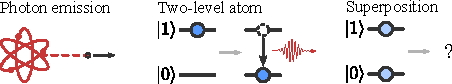
\includegraphics[width=0.7\textwidth]{lesson13/13-4_memory-first.pdf}
    \caption[First idea for memory]{Our first idea for a memory qubit is to use two energy levels of a system, such as ground and excited states of an atom.}
    \label{fig:13-memory-first}
\end{figure}

First, where is our qubit \ket{0} and \ket{1} in our quantum memory? Our quantum memory is a two-level system, and it has a ground state \ket{g}, and some excited state of higher energy which we can label \ket{e}. These are natural candidates for representing \ket{0} and \ket{1}. For example, Fig.~\ref{fig:13-memory-first} shows a two-level atom where $\ket{0}\equiv\ket{g}$ and $\ket{1}\equiv\ket{e}$. Now, how do we represent the flying qubit so that it works well with this memory qubit definition? One possibility is to use the presence or absence of a photon as a qubit, giving the definitions $\ket{0}\equiv\ket{\textrm{no photon},\ket{1}\equiv\ket{\textrm{photon}}}$.
We can see that if the atom decays from the excited state into its ground state, that is, it makes a transition from \ket{1} to \ket{0}, it emits a photon.

%\rdv{layout here isn't quite right, words in the middle should really be grouped with equations on the left}
\begin{equation}
\begin{array}{ll}
\text{memory qubit} & \text{flying qubit} \\

|0\rangle \equiv|g\rangle \quad \text { ground state } & \quad|0\rangle \equiv \mid \text {no photon}\rangle \\
|1\rangle \equiv|e\rangle \quad \text { excited state } & \quad|1\rangle \equiv \mid \text {photon}\rangle \\
\end{array}
\end{equation}

Now, how about coherences and superpositions? We can prepare our memory in a superposition of the ground state and the excited state by applying an appropriately timed energy pulse. If we use this state representation for memory, then our question is, "Well, what happens when we prompt the atom to emit a photon? Does it get emitted, or does it not get emitted? If it does get emitted, in what state will it be?" We see that the atom has a 50\% probability to be found in the ground state, where it cannot emit any energy. In that case, our photonic qubit will be in the \emph{no photon}, or \ket{0}, state. The atom also has a 50\% probability of being in the excited state, from where it can emit a photon. In this way, we can think about our photonic qubit as being in a superposition of \ket{0} and \ket{1}, or \ket{\textrm{no photon}} and \ket{\textrm{photon}}.
Since this this technique leaves the memory qubit in \ket{0}, we can say that it transfers the state \ket{+} from the atomic memory to the flying qubit. 

% \begin{figure}[t]
%     \centering
%     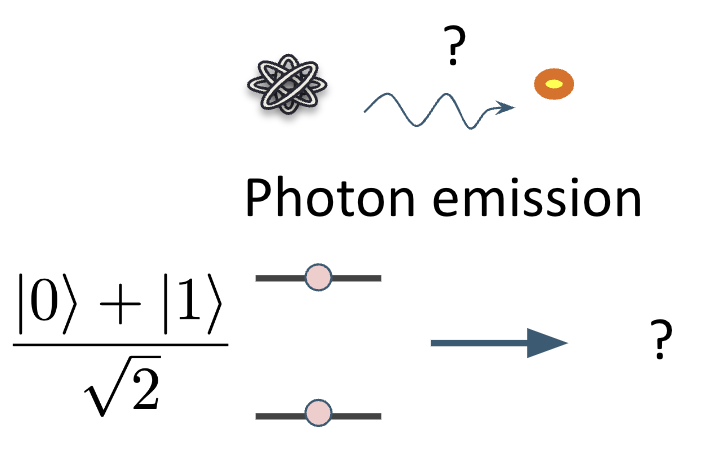
\includegraphics[width=0.7\textwidth]{lesson13/memory-first-idea-problem.png}
%     \caption[Problem with our first idea for memory]{Our first idea for a memory qubit appears to have a clean correspondence with the flying qubit, but then loss of the photon can make the state ambiguous.}
%     \label{fig:13-memory-first-problem}
% \end{figure}

\begin{figure}[t]
    \centering
    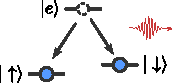
\includegraphics[width=0.3\textwidth]{lesson13/13-4_memory-second.pdf}
    \caption[Our second idea for memory]{Our second idea for a memory qubit is to use the post-decay spin of an atom. This allows us to use a polarized photon as a flying qubit robust against loss.}
    \label{fig:13-memory-second-idea}
\end{figure}

This is a very naive picture that demonstrates only some of the basic principles of how stationary and flying qubits interact. In real systems, things are a lot more complicated. In particular, when we look at this encoding of using two levels for our quantum memory, it is usable but it's not a very good qubit for communication. Due to the energy relaxation process, our excited state will eventually decay into a \ket{0}, destroying whatever state we had encoded into the quantum memory. Similarly, our choice of encoding for the flying qubit is not very good due to the attenuation of light in fiber. 
% We described it in some detail that as we send photons down a fiber, attenuation means they are very likely to be lost. 
If we are waiting for some message at the end of the fiber and we don't receive a photon, we cannot be sure if the original message was really \ket{\textrm{no photon}} (\ket{0}), or if the initial message was \ket{\textrm{photon}} (\ket{1}) and the photon just got lost along the way. So, we have to be a little bit more careful and think of a better, more robust way to encode our information.

What's our next choice for stationary memory qubit and flying qubit?

Consider the following atomic structure: we have two degenerate~\footnote{Meaning "having the same energy"; no moral weakness implied.} ground states, and we will label them as ground state up (\ket{\uparrow}) and ground state down (\ket{\downarrow}), as shown in Fig.~\ref{fig:13-memory-second-idea}. These can represent the two spins\index{spin} of our atom.
For our flying qubits, the matching state will be polarization, where \ket{0} will be represented by vertical polarization (\ket{V}), and \ket{1} will be represented by horizontal polarization (\ket{H}). 

% \rdv{layout here isn't quite right, words in the middle should really be grouped with equations on the left}
\begin{equation}
\begin{array}{ll}
\text{memory qubit} & \text{flying qubit} \\
|0\rangle \equiv|\uparrow\rangle \text { spin up } & |0\rangle \equiv|V\rangle \\
|1\rangle \equiv|\downarrow\rangle \text { spin down } & |1\rangle \equiv|H\rangle
\end{array}
\end{equation}

We prepare our atom initially in the excited state, then stimulate the atom to decay, either to the ground state with spin up, or to the ground state with spin down, each with 50\% probability.  If the atom decays into the spin up state, the emitted photon will be vertically polarized.  If the atom decays into the spin down state, the photon will be horizontally polarized.  The thing is, we can only see that a photon comes out, and we don't actually know into which ground state the atom decayed. We are effectively implementing the following transformation: we go from the excited state of the atom to a superposition of the atom being found in the spin up state and the spin down state. 
%If that's true, then the photon that gets emitted just happens to have a vertical polarization. On the other hand, if it decays into the other ground state given by spin down, then the photon will have a horizontal polarization. So really, what we are doing is we are obtaining the following superposition of two qubits (top right eq.). 
Moreover, since the state of the emitted photon depends on the final state of the atom, we now have an equal superposition of the atom being in the spin up state and the emitted photon being vertically polarized, and the atom being found in the spin down state and the photon being horizontally polarized. We can write this transformation as
\begin{equation}
\ket{e} \rightarrow \frac{\ket{\uparrow V}+\ket{\downarrow H}}{\sqrt{2}}
\end{equation}
where the up and down arrows represent the post-decay state of the atom and the letters represent the polarization of the emitted photon.  (The left hand side of the equation has no photon, only the state of the atom.) In this way, we are entangling the flying photon with the stationary qubit of the memory.

Fig.~\ref{fig:13-MIM-energy} brings this all back to a concrete representation of our Bell-state analyzer. We have drawn this before very abstractly, but now we have a much better idea how to make it work in practice. In the middle are the two single-mode fibers. On the left are the two quantum memories at our two repeater nodes, separated by some distance, represented by their energy level diagrams. Each memory is prepared initially in the excited state \ket{e}, which decays into one of its ground states, either spin up \ket{\uparrow} or spin down \ket{\downarrow}. We don't know which state it decays into, leaving us with a flying photon that is entangled with its respective memory. These flying photons travel through the single mode fibers, then hit the central beam splitter, where (if all goes well) they interfere and we perform a Bell-state measurement using the other two beam splitters and the four detectors. In this way, we can establish link-level entanglement between the atomic memories sitting at the ends of the link. This is exactly the scheme that we have described previously for a midpoint-interference-memory (MIM) link. In terms of physics is the same as a direct memory-to-memory connection (MM).

\begin{figure}[t]
    \centering
    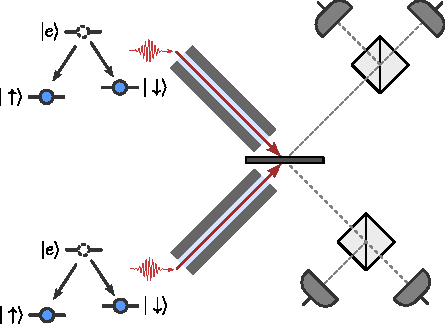
\includegraphics[width=0.7\textwidth]{lesson13/13-4_MIM_with_energy_levels.pdf}
    \caption[MIM with energy levels]{A different view of an MIM link. On the left are the energy level diagrams for the qubits, which decay into a superposition of two states while emitting photons entangled with the memories. On the right is a large view of the Bell state analyzer with three beam splitters and four photon detectors.}
    \label{fig:13-MIM-energy}
\end{figure}




\newpage
\begin{exercises}
\exer{Consider the following quantum state:}
\begin{equation*}
\ket{\psi} = \frac{\sqrt{3}}{2}\ket{0} + \frac{1}{2}\ket{1}
\end{equation*}
\subexer{Find the probability of measuring a zero.}
\subexer{Find the probability of measuring a one.}


\end{exercises}

\newpage
\section*{Quiz}
  \addcontentsline{toc}{section}{Quiz}

%\section{Learning more}

\section*{Further reading chapters 11-13}
  \addcontentsline{toc}{section}{Further reading chapters 11-13}

{\bf Chapter 11}

For those interested in how submarine fiber optic cables are made, laid and operated we recommend the following online article found here.\rdv{where???}

Our discussion of mode dispersion closely followed Section 5.6 of Hecht’s textbook and we encourage you to read it for the extra details that can be found in the book.

A qualitative review of classical amplifiers (with just the right amount of technical detail) can be found here:

Emmanuel Desurvire, The Golden Age of Optical Fiber Amplifiers, \emph{Physics Today} 47, 20 (1994).

Unfortunately, this article is behind a paywall so you will have to use your university’s online system to access it.

{\bf Chapter 12}

Quantum repeaters are the "bread and butter" of quantum networks. The names Wolfgang D\"ur and Hans Briegel cannot be mentioned often enough in the history of repeaters. Those interested in the paper that introduced the idea of a quantum repeater (and are not scared off by maths) might have a look here:

Hans J. Briegel, Wolfgang Dür, Juan I. Cirac, Peter Zoller, Quantum repeaters: The role of imperfect local operations in quantum communication, \emph{Physical Review Letters} 81, 5932, 1998~\cite{briegel98:_quant_repeater}.

The paper is behind a paywall and needs to be accessed through your university’s library online services. An earlier version of the paper can be accessed openly here.

One place to learn more is Prof. Van Meter's previous book,\\
Rodney Van Meter, \emph{Quantum Networking}, Wiley-ISTE, 2014~\cite{van-meter14:_quantum_networking}.



{\bf Chapter 13}

A great popular article about the physical layer components of quantum networks can be found here:
Dan Hurley, The quantum internet will blow your mind. Here’s what it will look like, \emph{Discover Magazine}, 2020.

Another fantastic review of physical layer components can be found here:

Nicolas Sangouard, Christoph Simon, Hugues de Riedmatten, Nicolas Gisin, Quantum repeaters based on atomic ensembles and linear optics, \emph{Review of Modern Physics} 83, 33, 2011~\cite{sangouard2011quantum}.

Again, the published version is behind a paywall but the pre-publication version can be accessed for free here. Be warned though, this paper starts with an excellent introduction but the technical details ramp up quickly after that and rely on good grasp of quantum optics. So if you get lost after the introduction, don’t worry. You can come back to those parts later.
